\documentclass[11pt,a4paper]{article}
\usepackage[utf8]{inputenc}
\usepackage[T1]{fontenc}
\usepackage{lmodern}
\usepackage{arxiv}
\usepackage{dsfont}
\usepackage{amsmath}
\usepackage[backend=biber]{biblatex}

% --- Core packages
\usepackage{booktabs}
\usepackage{graphicx}
\usepackage{float}
\usepackage{amsfonts}
\usepackage{amssymb}
\usepackage{nicefrac}
\usepackage{microtype}
\usepackage{lipsum}
\usepackage{comment}

% --- Links (load hyperref LAST among basic packages)
\usepackage{url}
\usepackage{doi}
\usepackage{hyperref}

\usepackage{xcolor}
\usepackage{lastpage}
\cfoot{\small\color{gray}Page \thepage\ of \pageref{LastPage}}

% --- Tables, lists, formatting
\usepackage{caption}
\captionsetup{labelfont=bf, textfont=it}
\usepackage{enumitem}

% --- Code + colors
\usepackage{listings}

% --- Line spacing
\usepackage{setspace}
\onehalfspacing

% --- Bibliography (biblatex version)
\addbibresource{references.bib}

% --- Title metadata (Configured for the header)
\hypersetup{
pdftitle={TASK 2: Predicting Frustration from Heart Rate Signals},
pdfsubject={DTU 02445},
pdfauthor={Yutao Zhang},
pdfkeywords={}
}

\begin{document}

\begin{titlepage}
    \centering
    \vspace*{0.8cm}

    {\LARGE \textsc{Technical University of Denmark} \par}
    \vspace{0.2cm}
    {\large Artificial Intelligence and Data \par}

    \vspace{1.2cm}

    
\includegraphics[width=3.5cm]{DTU-logo.png}

    \vspace{1.2cm}

    \rule{\textwidth}{1pt}
    \vspace{0.5cm}

    {\huge TASK 2: Predicting Frustration from Heart Rate Signals \par}

    \vspace{0.3cm}
    \rule{\textwidth}{1pt}

    \vspace{2.0cm}

    {\Large
    Yutao Zhang\\
    Student Number: 255854
    \par}

    \vspace{1.5cm}

    {\large
    \textbf{Course:}\\
    Project in statistical evaluation of Artificial Intelligence and Data (02445)
    \par}

    \vfill
\end{titlepage}

\setcounter{page}{1}

\section*{Introduction}

Frustration is a common but disruptive emotional response during collaborative problem-solving tasks. Self-reported emotional states are subjective and hard to collect mid-task, so physiological signals offer a useful, continuous alternative: heart rate (HR), recorded via wearable sensors, gives an objective window into autonomic arousal. This study tests whether HR summary statistics can predict self-reported frustration during an interactive puzzle task and generalize to people the model has not seen before, rather than building a model personalized to each individual. To keep the performance estimate honest on this small sample, nested Leave-One-Subject-Out cross-validation is used throughout.

\section{Methods}

\subsection{Data and Target Binarization}

This study analyzes a 168-row subset of the EmoPairCompete dataset: 14 individuals, each contributing 12 observations from a balanced design of 4 rounds and 3 phases. Each row contains six heart rate statistics (\texttt{HR\_Mean}, \texttt{HR\_Median}, \texttt{HR\_std}, \texttt{HR\_Min}, \texttt{HR\_Max}, \texttt{HR\_AUC}), the categorical \texttt{Round} (1--4) and \texttt{Phase} (1--3), and a self-reported frustration score (0--8).

This is framed as classification rather than regression. The 0--8 score is a subjective self-report, not a precisely measured continuous quantity, and people likely calibrate it differently from one another, so treating it as interval-scaled would assume more precision than the data has. The scores are also heavily skewed low (median 2, mean 2.3; only 6\% of rows are 6 or above), leaving little signal for a regression model to learn from in the upper range with just 14 individuals. Classification also matches the practical goal directly, since flagging distress is itself a binary decision, whereas a regression output would still need a threshold applied afterwards to be useful.

Within that classification framing, a binary rather than a multi-class target is used for two reasons. With only 168 rows from 14 people, splitting into more classes would leave too few examples per class to train reliably, especially for the ANN. Collapsing the scale to a single state-shift also reduces the reporting-noise problem above and matches the practical goal of flagging the moment someone crosses into distress, rather than tracking fine-grained emotional increments.

Because these self-reports are subjective,\footcite[Page 9, Paragraph 3 (under "Phase Analysis")]{das2024} the target is binarized as $\texttt{Frustrated\_binary} = 1$ if $\texttt{Frustrated} \geq 3$, else $0$. This threshold is supported by the data: mean frustration is low during the resting (1.21) and recovery (1.89) phases, but rises to 3.77 during the active puzzle-solving phase.\footnote{See Appendix~\ref{fig:Empirical_threshold}. A threshold of 3 cleanly separates the task-induced state from baseline calm.}

\subsection{Feature Selection and Engineering}

Raw HR values were compared against individual-specific z-scores, where each feature is centered on that person's own mean and scale. This reordered feature importance: \texttt{HR\_Mean} and \texttt{HR\_Median} became the strongest predictors, while \texttt{HR\_Max} and \texttt{HR\_std}, the strongest in the raw data, dropped to the weakest, suggesting that raw variance partly reflects movement artifacts rather than affect. \texttt{HR\_Min} was the weakest predictor in both versions and was dropped.\footnote{Each person's z-score uses that person's own mean and standard deviation computed from all 12 of their rows, which a genuinely new person under leave-one-subject-out would not yet have. Recomputing these statistics from only each person's four resting-phase (\texttt{phase1}) rows, a calibration window that never touches a frustration-relevant row, left logistic regression's pooled balanced accuracy and ROC-AUC essentially unchanged ($0.597\to0.576$ and $0.607\to0.577$), so this does not appear to inflate the reported performance.}

The final feature set is five z-scored HR features (\texttt{Mean}, \texttt{Median}, \texttt{std}, \texttt{Max}, \texttt{AUC}): 5 columns in total. \texttt{Phase}, \texttt{Round}, and \texttt{Puzzler} are not used as model inputs: they describe the experimental design (which segment, repetition, and role a row comes from) rather than a physiological signal, and the model is meant to learn from heart rate, not from recognizing the experimental setup. \texttt{Individual} and \texttt{Cohort} are likewise never inputs; they are used only to define the cross-validation groupings (Section 2.3), not as features to learn from.

\subsection{Classification Models and Cross-Validation}

Two models spanning interpretable to flexible are compared. \textbf{Logistic regression} is a linear model: each feature's effect on the log-odds of frustration is a single, readable coefficient. It is also the model class built specifically for binary outcomes, fitting a Bernoulli likelihood directly, rather than a general-purpose model merely adapted to classification. The \textbf{ANN} is a single hidden-layer multi-layer perceptron, able to capture non-linear feature interactions a linear model cannot, with its size and regularization tuned to limit overfitting on a dataset this small. Both models, the preprocessing pipeline, and the cross-validation splitters described below were implemented in Python with the scikit-learn library (Pedregosa et al., 2011).

The dataset's repeated-measures structure (12 rows per individual) rules out a random train-test split, since a model could partly "recognize" a person from their own baseline HR rather than learning a pattern that generalizes. The 14 individuals also come from two cohorts (8 and 6 individuals, with no individual in both); holding out a full cohort at a time would leave too few people for reliable inner-loop tuning, so individuals rather than cohorts are held out, which still tests generalization to someone absent from training. Nested Leave-One-Subject-Out (LOSO) cross-validation is therefore used: an outer loop holds out one individual at a time across 14 folds, while an inner \texttt{StratifiedGroupKFold} loop on the remaining 13 individuals selects hyperparameters (\texttt{GridSearchCV} for logistic regression's $C$ and \texttt{class\_weight}; \texttt{RandomizedSearchCV} for the ANN's architecture and learning rate) and the decision threshold that maximizes balanced accuracy on the inner folds. Pooling all 14 outer folds gives 168 out-of-fold predictions, one per row, each from a model that never saw that person during training.

\section{Results}

Logistic regression converged on $C=0.001$ with \texttt{class\_weight='balanced'} -- strong regularization that shrinks all five HR coefficients toward zero; the ANN converged on a single 16-unit hidden layer (\texttt{relu} activation, $\alpha \approx 0.047$, batch size 32, learning rate $\approx 2.4\times10^{-3}$).

\begin{table}[H]
\centering
\caption{Pooled nested-LOSO out-of-fold classification metrics (168 predictions), five HR features only. Balanced accuracy is shown with a 95\% cluster-bootstrap confidence interval (resampling individuals, 2000 resamples).}
\vspace{0.1cm}
\begin{tabular}{lccc}
\toprule
Model & Accuracy & Balanced Accuracy [95\% CI] & ROC-AUC \\
\midrule
Baseline (majority class) & 0.625 & 0.500 & 0.500 \\
Logistic Regression & 0.595 & 0.597 [0.516, 0.684] & 0.607 \\
ANN                  & 0.506 & 0.506 [0.446, 0.581] & 0.448 \\
\bottomrule
\end{tabular}
\end{table}

Neither model clearly beats the majority-class baseline (Table 1): logistic regression's balanced-accuracy 95\% confidence interval ([0.516, 0.684]) only barely excludes the 0.50 chance level, and the ANN's ([0.446, 0.581]) includes it outright, with a ROC-AUC of 0.448, worse than random guessing. Both models agree that \texttt{HR\_Mean} is the strongest of the five features (logistic regression's largest coefficient; the ANN's largest permutation importance, $0.092$, with \texttt{HR\_AUC} a distant second at $0.076$), but logistic regression's coefficients are all small ($\leq 0.012$) under the heavy regularization the inner CV selected -- itself a sign that the inner loop found little signal worth fitting.

A paired Wilcoxon signed-rank test on per-individual balanced accuracy ($n=14$) found no detectable difference between the two models ($p=0.249$); with only 14 individuals the test has low power, so this is read as no detectable difference rather than proof of equivalence. A cluster-bootstrap 95\% CI on the paired difference (LogReg $-$ ANN $=0.090$, 95\% CI [$-0.012$, $0.198$]) and McNemar's test on the pooled predictions ($p=0.044$) both point toward logistic regression doing modestly better, though McNemar assumes independent rows, which the repeated-measures structure violates, so the per-subject Wilcoxon test remains the primary, more trustworthy read.

\section{Discussion}

Nested LOSO cross-validation was essential here: with only 14 individuals, any split that mixes one person's rows across train and test would overstate how well a model generalizes to someone new.

Logistic regression numerically outperforms the ANN on every metric (Table 1): its balanced accuracy and ROC-AUC sit a little above chance, while the ANN's barely move from $0.50$ and its ROC-AUC even dips below it. With only 14 individuals, the ANN has comparatively many parameters relative to the available signal, so its near-chance performance likely reflects overfitting the inner-loop hyperparameter search to noise rather than a genuine inability to use heart rate. The gap is not significant by the per-subject Wilcoxon test ($p=0.249$), but the bootstrap CI on the difference nearly excludes zero and McNemar's cross-check does cross the conventional threshold ($p=0.044$), so the safer reading is a real if modest edge for logistic regression, not that the two models are interchangeable. Both models independently rank \texttt{HR\_Mean} as the strongest HR feature, the one piece of convergent, model-independent evidence that heart rate carries some signal here, however weak. Read together, these results look less like a failed prediction task and more like a validation scheme working as intended: a 14-person, repeated-measures dataset with infrequently-elevated, self-reported frustration scores is not expected to support strong prediction from five HR summary statistics, and an honest cross-validation scheme should show that plainly.

Logistic regression is therefore the preferred model: it scores better on every metric, has a convex and deterministic fit that is not sensitive to random initialization the way the ANN's is, and is fully interpretable as the model class built specifically for binary outcomes. Without any demonstrated benefit from the ANN's extra complexity, and with the small sample making that complexity riskier rather than safer, the simpler, auditable model is the more appropriate choice here.

\textbf{Reflections on the binarization threshold.} A cutoff of 3 favors sensitivity to early signs of distress over specificity; a cutoff of 4 would trade some of that sensitivity for fewer false positives, since engagement at a score of 3 is not always genuine distress.

\clearpage
\printbibliography[title={References}]


\section{Appendix}

\begin{figure}[H]
    \centering
    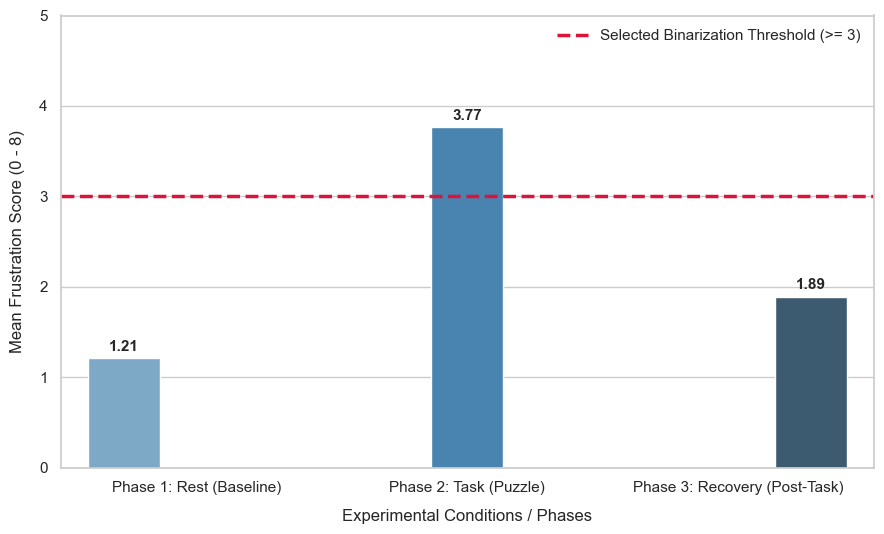
\includegraphics[width=1\linewidth]{Empirical_threshold.png}
    \caption{Empirical Support for Frustration Cut-off Threshold}
    \label{fig:Empirical_threshold}
\end{figure}
\clearpage

\label{Code}
\textit{The code used in the task can be found in the GitHub repository at:} \href{TODO-INSERT-REPO-URL}{TODO: insert repository URL}.

%husk at ændre



\section*{Declaration of AI use}
\small
I/we have used AI for the following tasks:

\setlist[itemize]{noitemsep, topsep=2pt, partopsep=0pt, parsep=0pt}

\textbf{Writing / Text Generation}
\begin{itemize}
  \item[$\blacksquare$] Rephrase or improve wording, grammar, or style.
  \item[$\square$] Summarize external sources or content.
  \item[$\blacksquare$] Check or enhance logical flow or structure of the report.
  \item[$\blacksquare$] Draft sections of the report.
\end{itemize}

\textbf{Research \& Information Gathering}
\begin{itemize}
  \item[$\blacksquare$] Find primary or secondary sources (papers, articles, data).
  \item[$\blacksquare$] Serve as a primary source of information or data.
  \item[$\square$] Summarize or extract key points from sources.
  \item[$\square$] Interpret or explain findings from literature.
\end{itemize}

\textbf{Idea Generation / Brainstorming}
\begin{itemize}
  \item[$\square$] Generate initial ideas or hypotheses for experiments or projects.
  \item[$\square$] Propose alternative approaches, solutions, or interpretations.
  \item[$\square$] Suggest research questions or objectives.
  \item[$\blacksquare$] Identify potential limitations or challenges.
\end{itemize}

\textbf{Design of Experiments / Methodology}
\begin{itemize}
  \item[$\square$] Design experiments or workflows.
  \item[$\blacksquare$] Optimize parameters or settings for experiments.
  \item[$\square$] Propose control conditions or comparison groups.
  \item[$\blacksquare$] Assist with experimental planning or sequencing of tasks.
\end{itemize}

\textbf{Computer Code / Programming}
\begin{itemize}
  \item[$\blacksquare$] Debug code or identify errors.
  \item[$\blacksquare$] Automate repetitive coding tasks.
  \item[$\blacksquare$] Explain programming concepts, algorithms, or logic.
  \item[$\blacksquare$] Optimize or refactor code for efficiency or readability.
  \item[$\blacksquare$] Generate code snippets or full programs (\textit{not main code}).
\end{itemize}

\textbf{Figures, Illustrations, \& Visualizations}
\begin{itemize}
  \item[$\square$] Propose visual design or layout of figures.
  \item[$\square$] Edit or format images for the report.
  \item[$\square$] Generate diagrams, schematics, or drawings.
  \item[$\blacksquare$] Create or enhance graphs, plots, or charts.
\end{itemize}

\textbf{Data Analysis \& Interpretation}
\begin{itemize}
  \item[$\square$] Process or clean data.
  \item[$\blacksquare$] Perform statistical analyses.
  \item[$\blacksquare$] Interpret results or trends.
  \item[$\blacksquare$] Generate tables or visual summaries of data.
\end{itemize}

\textbf{Other Uses of AI}
\begin{itemize}
  \item[$\square$] Other (please specify):
  \item[$\blacksquare$] Support use of latex.
\end{itemize}

\textbf{Confirmation of No Inappropriate Use}
\begin{itemize}
  \item[$\blacksquare$] I have not submitted AI-generated work as entirely my own without disclosure.
  \item[$\blacksquare$] I have not used AI to fabricate or invent data, results, or references.
  \item[$\blacksquare$] I have not used AI to plagiarize or copy others' work without correct attribution.
  \item[$\blacksquare$] I have not used AI to violate copyright, GDPR, or confidentiality requirements.
  \item[$\blacksquare$] I have not used AI to bypass safety, ethical, or legal guidelines related to the project.
\end{itemize}

\normalsize
\end{document}
